\chapter{Teorie}

Semestrální práce se zejména zabývá problematikou \acs{MIR}. Popsánou v kapitole (!doplnit kapitolu!).
Důležitou roli zde hraje i úvaha nad realizací světelných animací.
Je důležité aby bylo přemýšleno nad principem reakce světelných animací na hudbu.
Nabízejí se otázky jak by měla daná animace reagovat na konkrétní děj skladby.
Jakým způsobem navrhnout strukturu \dots

V táto části je popsána teorie zpracování hudební nahrávky pomocí známých algoritmů jako je například \acs{FFT} (\acl{FFT}) 
či nabízené možnosti strojového učení. Struktura a možnosti systému Spectoda pro generování interaktivních světelných animací.
Uměleckou částí, jak by měla animace prezentovat hudbu.

\section{MIR - Music information retrieval}
    Music information retrieval je interdisciplinární vědní obor sostředící se na získávání infromací z hudebních nahrávek.
    Jsou zde kombinovány znalosti mnoha oborů jako jsou muzikologie, psychoakustika, strojové učení, zpracování signálů a další. 
    

    Výstup jeho výzkumu je využíván populárními technologiemi. 
    Jednou z aplikací je personalizované doporučování hudebních skladeb, která se nachází v moderních streamovacích platformách.
    Další využítí je v programech pro mixování hudby používaných diskžokeji k plynulejší práci díky alanýze tempe a klíčových částí skladby.
    Tyto technologie se nachází v mnoha dalších aplikacích a s šířením se digitálního audia jejich důležitost stále poroste.
    \cite{lidy09:448[TUW-181186]}\cite{a_new_companion_to_digital_humanities}
    
    \subsection{Historie}
    \acs*{MIR} se začíná objevovat koncem devatenáctého a začátkme dvacátého století s příchodem moderních statistických metod.
    V některých univerzitách tyto statistické metody začínají aplikovat na hudebu.
    Ze začátku díky špatné dostupnosti počítačů se jedná spíše o ruční přepisování tabulatur přímo z hudebních partitur.
    Následně se ze zjištěných rysů snažili specifikovat stylové chrakteristiky.  
    S příchodem počítačů do výzkumných laboratoří v letech 1960 až 1970 se začalo více soutředit na počítačovou analýzu hudeby.
    V těchto letech se poprvé začaly objevoat nyní známé termíny jako \uv{\it computational musicology} a \uv{\it music information retrieval}
    První oblastí výzkumu bylo získávání rytmu hudbení nahrávky a z důvodu nízké popularity se výzkum zpomalil.
    Tento trend následoval až do roku 1990 kdy vázkumu \acs*{MIR} pomohly dvě věci.
    První z nich bylo velké zvětšování lehce dostupné hudby a druhým z důležitých bodů byl nárůst výpočetního výkonu počítačů.
    Díky těmto bodům se stal výzkum dostupnější a jednodužší na realizaci.

    Poté v říjnu roku 2000 bylo uspořádáno první mezinárodní symposium soustředící se na \acs*{MIR}.
    Následně díky těmto pokrokům vznika celosvětová skupina \acs{ISMIR} (\acl{ISMIR}).
    Zanedlouho naté vznikla další skupina \acs{MIREX} (\acl{MIREX}). Jedná se o skupinu vědců která se schází pravidelně každý rok a řeší problematiku \acs{MIR}.
    
   \subsection{Řetězec zpracování - pipeline}

    Téměř standardně využívaný řetězec procesů v aplikacíc \acs{MIR} je popsána níže. 

    Jako vstupní data se využívají zejména hudební informace v digitální potobě.
    Tyto data se rozlišují do více typů. Mohou to být obrázky představující digitální formu zápisu hudby pomocí symbolů (not).
    Dalším možným typem je "digitální hudba", představovaná zápisem v \acs{MIDI} notách.
    V této práci budou jako vstupní data yvužívány digitální hudební nahrávky ("digitální audio"). 

    Pokud jsou vstupní data komplexní na začátku je v řetězci zařezen blok předzpracování, která se stará o komprimaci vstupních singálů.
    U hudebních signálů se jedná například o konverzi stereo signálů na mono signál
    a jeho následnou komprimaci popsanou více v bodě 
    %TODO: odkaz na bod audio

    Dalším bodem v řetězci je extrakce vlastností signálu. 
    Zde je je nastaven poměr mezi vlastnostmi důležitými pro strojové učení lidskou expertní znalost.
    Poměr mezi těmito vlastnostmi závisí na aplikaci pro kterou je algoritmus určen.
    Ná základě získaných vlastností je nastavena struktura algoritmu pro odvození výsldných parametrů.

\begin{figure}[H]
    \centering
    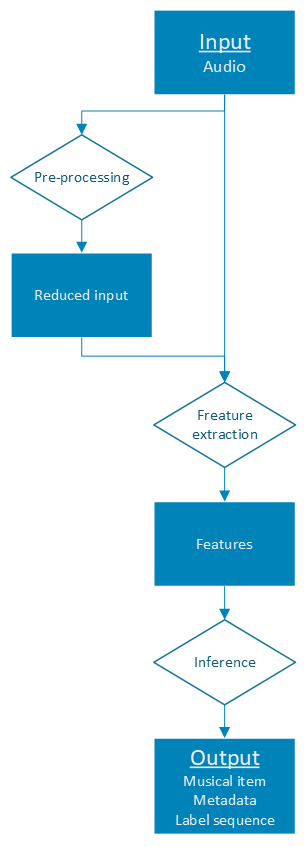
\includegraphics[width = 0.4\linewidth]{obrazky/MIR-diagram.png}
    \caption{Řetězec procesů MIR \cite{a_new_companion_to_digital_humanities}}
    \label{fig:MIR_diagram}
\end{figure}

    Zpracování audio signálů je již dvě desetilétí hlavním trendem výzkumu \acs*{MIR}.
    Je to přirození tím, že zde není téměř žádná přirozená hranice a je možné téměř vše.
    Právní podmínky jsou zde příznivé a vědecké instituce nemají problém pro svou práci získat velké množství materiálu chráněného autorským právem.
    Z důvodu velké komplexsnosti vstupních signálů se využívá několik technik komprimaca signálů kterými jsou. 
    Slučování vícekanálových nahrávek do mono sginálu. Převzorkování signálu na nižší vzorkovací kmitočty,
    a rozložení signálu na krátké překrývající se úseky ze kterých mohou být nezávisle extrahovány jejich vlastnosti. 
    Výsledkem je kolekce paralelně složených sekvencí hodnot vlastností, které se následně použijí pro odvozování (inference).

  \begin{table}[H]
    \centering
    \begin{tabular}{|p{0.07\linewidth} | p{0.31\linewidth} | p{0.27\linewidth} | p{0.25\linewidth}|}
        \hline
        {\bf Data}                 & {\bf Vyhledávání informací} & {\bf Klasifikace a odhad} & {\bf Sekvenční značení}\\
        \hline
        Audio                      & Identifikace skladby,
                                     Řazení,
                                     Měření podobnosti,
                                     Získání otisku,
                                     Generování seznamu skladeb
                                   & Identifikace umělce a skladatele,
                                     Žánr a nálada,
                                     Určení tempa
                                   & Extrakce melodie,
                                     Odhad akordů,
                                     Detekce nástupů,
                                     Segmentace                   \\
        \hline
    \end{tabular}
    \caption{Typické procesy na základně vstupních a výstupních dat.}
    \label{tab:MIR_typicke_procesy}
  \end{table}

  %TODO: současné problémy


  \section{Parametrizace hudebních nahrávek}
  V této kapitole je popsán audio signál. Jak vzniká, jeho reprezentace v číslicovám zpracování a základní principy práce s audiosignálem.
  V bodech \ref{sec:Frekvence} až \ref{sec:Barva} jsou popsány parametry získávané z audio signálu. %TODO: doplnit správné reference
  Získané parametry slouží pro přesnější popis skladby. \cite{fundamental_of_music_processing}

  \subsection{Reprezentace audio signálů}
  Hudba může být reprezentována spoustou forem. 
  Jako tradiční médium pro její ukládání ještě před vznikem záznamu sloužily vždy noty a další typy zápisů pomocí symbolů.
  Výsledné hudební dílo ale představuje mnohem více než počáteční notový zápis.
  Každý hudebník a hudební nástroj do skladby dodává svou unikátnost.
  Při hře se noty začnou proměňovat v harmonické zvuky, hladké melodie a nástroje vzájemně rezonují. 
  Každý z hudebníků do skladby přináší svou interptretaci. Jinak reagují na tempo zvýrazňují odlišné noty a liší se jejich artikulace.
  Všechny tyto proměnné ve výsledku způsobují, že dílo není jen mechanické přehrání napsané partitury.
  Jeho součástí se stává unikátní přednes.

  Při pohledu z fyzikálního hlediska důsledkem interpretace díla vznikají zvukové vlny šířící se vzduchem.
  Tyto vlny jsou reprezentovány kmítáním atomů plynu způsobující změny tlaku svým zhušťováním a zřěďováním. Při vlnění nedochází k přenosu hmotných částit.
  Záznamem šířících se zvukových vln získáváme audio signál.
  Pojmem audio je označován řetězec sloužící k záznamu, přenosu a reprodukci zvuků v mezích lidského slyšení. 
  Avšak v audio signálu se už nenachází přesná reprezentace not a jejich paramterů jako jsou čas nástupu, tón, délka trvání, dynamika.
  Díky tomu je analýza hudebních signálů obtížným úkolem a je ovlivněna reprezentací interpreta akustikou prostoru a vnímáním posluchače.
  Popsanými problémy se zabývá samostatný vědní obor s názvem psychoakustika.
  Nejdůležitějšími parametry audio signálu které jsou podrobně popsány níže definujeme: frekvence, výška tónu, dynamika, intenzita, hlasitost a také barva.


  \subsection{Časová oblast}
  Základní reprezentací audio signálu je tzv. zobrazení v \textbf{časové oblasti}.
  V časové oblasti číslicový signál představují vzorky. Jednotlivé vzorky udávají hodnotu signálu v daném čase.
  Počet vzorků nám určuje vzorkovací frekvence signálu. Důležé pravidlo pro vzorkování signálu je popsáno rovnicí č. \ref*{rov:vzorkovaci_teorem}
  
  \begin{equation}
    f_{vz} > 2 * f_{max}
    \label{rov:vzorkovaci_teorem}
  \end{equation}

  kde $f_{vz}$ je vzorkovací frekvence a $f_{max}$ je maximální frekvence v audio signálu.  
  Pokud jednotlivé vzorky zobrazíme graficky získáme průběh amplitudy signálu viz obrázek č.\ref*{fig:Waveform}

  \begin{figure}[H]
    \centering
    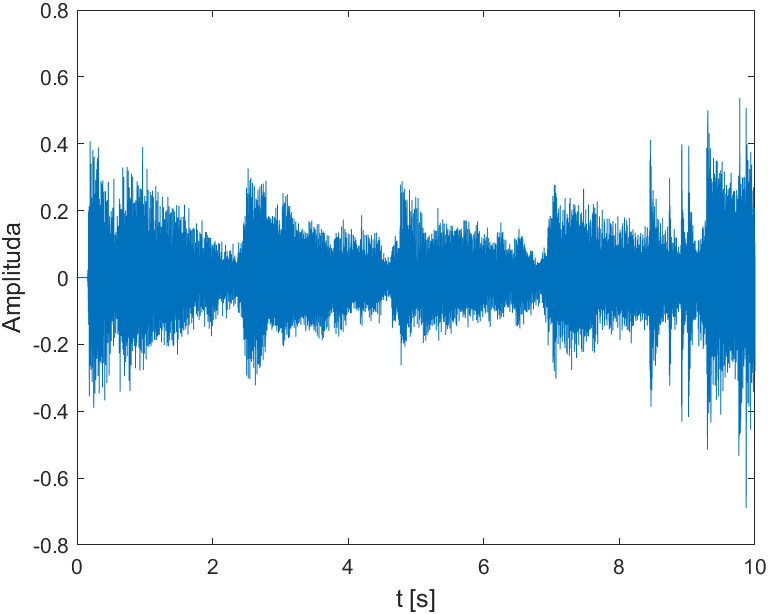
\includegraphics[width = 0.8\linewidth]{obrazky/Waveform.png}
    \caption{Zobrazení časového průběhu signálu}
    \label{fig:Waveform}
  \end{figure}

  Tato reprezentace audio signálu poskytuje informace o amplitudě signálu. Čili je z ní možno vyčíst například dynamiku skladby, začátky a konce not.
  
  \subsection{Frekvenční oblast}
  Pro získání více informací o hudebním díle je zobrazení v časové oblasti nedostatečné.
  Proto se využívá tzv. zobrazení ve \textbf{frekvenční oblasti}.

  V časové oblasti se zobrazuje frekvenční spektrum signálu.
  Toto spektrum představuje rozložení původní části signálu na jednotlivé harmonické frekvence reprezentující zpracovávaný signál.
  V grafu jsou poté zobrazy frekvenční složky se kterých se signál zkládá viz obrázek č.\ref*{fig:Bass_tone}.

  \begin{figure}[H]
    \centering
    \begin{subfigure}[b]{0.8\linewidth}
        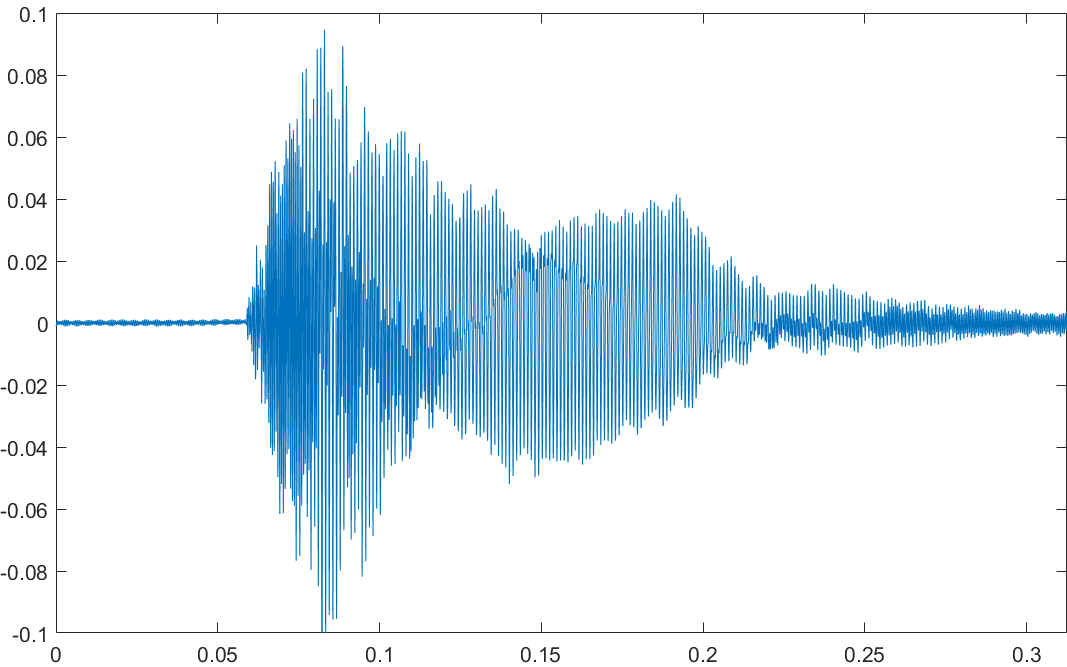
\includegraphics[width = \linewidth]{obrazky/Piano_tone_waveform.png}
        \caption{Časová oblast}
    \end{subfigure}
    \begin{subfigure}[b]{0.8\linewidth}
        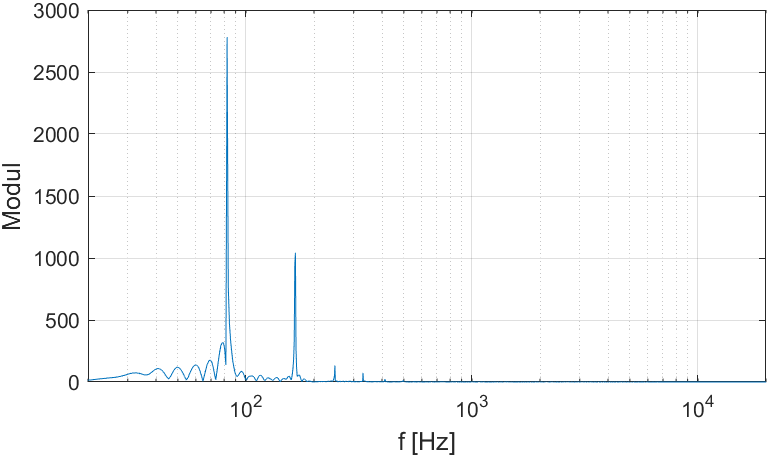
\includegraphics[width = \linewidth]{obrazky/Bass_tone_spectrum.png}
        \caption{Frekvenční oblast}
    \end{subfigure}
    \caption{Reprezentace tónu E zahraného na basovou kytaru.}
    \label{fig:Bass_tone}
\end{figure}
  
  Jako nzorný důvod proč je transformace do frekvenční oblasti přínosná je dán příklad. Na nástroj je zahrán tón, který je nahrán. 
  V časové oblasti je možné určit délku tónu a jeho průběh podle ADSR obálky popsané v bodě č. \ref*{sec:Barva}.
  Pokud je ale potřeba zjistit výšku tónu a určit notu, tak je to téměř nemožné.
  Díky transformaci do frekveční oblasti je patrná fundementální harmonická frekvence tónu.
  Tato frekvence udává výšku tónu a je tak možné stanovit notu která byla zahrána.

  Pro získání frekvenčního spektra signálu je třeba transformovat signál s časové oblasti.
  K tomu se využívá \textbf{Fourierovy transformace}. 

  Hlavní pilířem Fourierovy transformace je, že každý periodický signál je možné rozložit na součet někonečně mnoha sinusových signálů s různou amplitudou a fází.
  Toho je poté pomoí matematickýh postupů docílit.
  Analyzující signál je rozložen na jeho frekvenční složky udávané amplitudou a fází viz obrázek č.\ref*{fig:Bass_tone}.
  Jako další grafické zobrazení časové oblasti hudebního signálu se pro jeho analýzu využívá spektrogramu.
  % Spektrogram zobrazuje frekvenční složky signálu v závislosti na čase. Modul těchto složek je pak udáván barevnou škálou.
  % Spektrogram je zobrazen na obrrázku č. %TODO: popsat spektrogram zde nebo jinde? a popsat? 


  \subsection{DFT - Diskrétní Fourierova transformace}

  Pokud jsou signály zpracovávány pomocí výpočetních procesorů,
  tak může být uložen pouze omezený počet parametrů signálu.
  To znamená, že analogový signál spojitý v čase musí být převeden na signál digitální tvz. signál diskrétní, který je není spojitý v čase. 
  Diskrétní signál je potom vhodný pro číslicové zpracování.
  Důsledkem toho bylo nutné odvodit algoritmus \acs{DFT} přizpůsobený právě pro zpracování diskrétních signálů s konečným počtem hodnot.

  \begin{figure}[H]
    \centering
    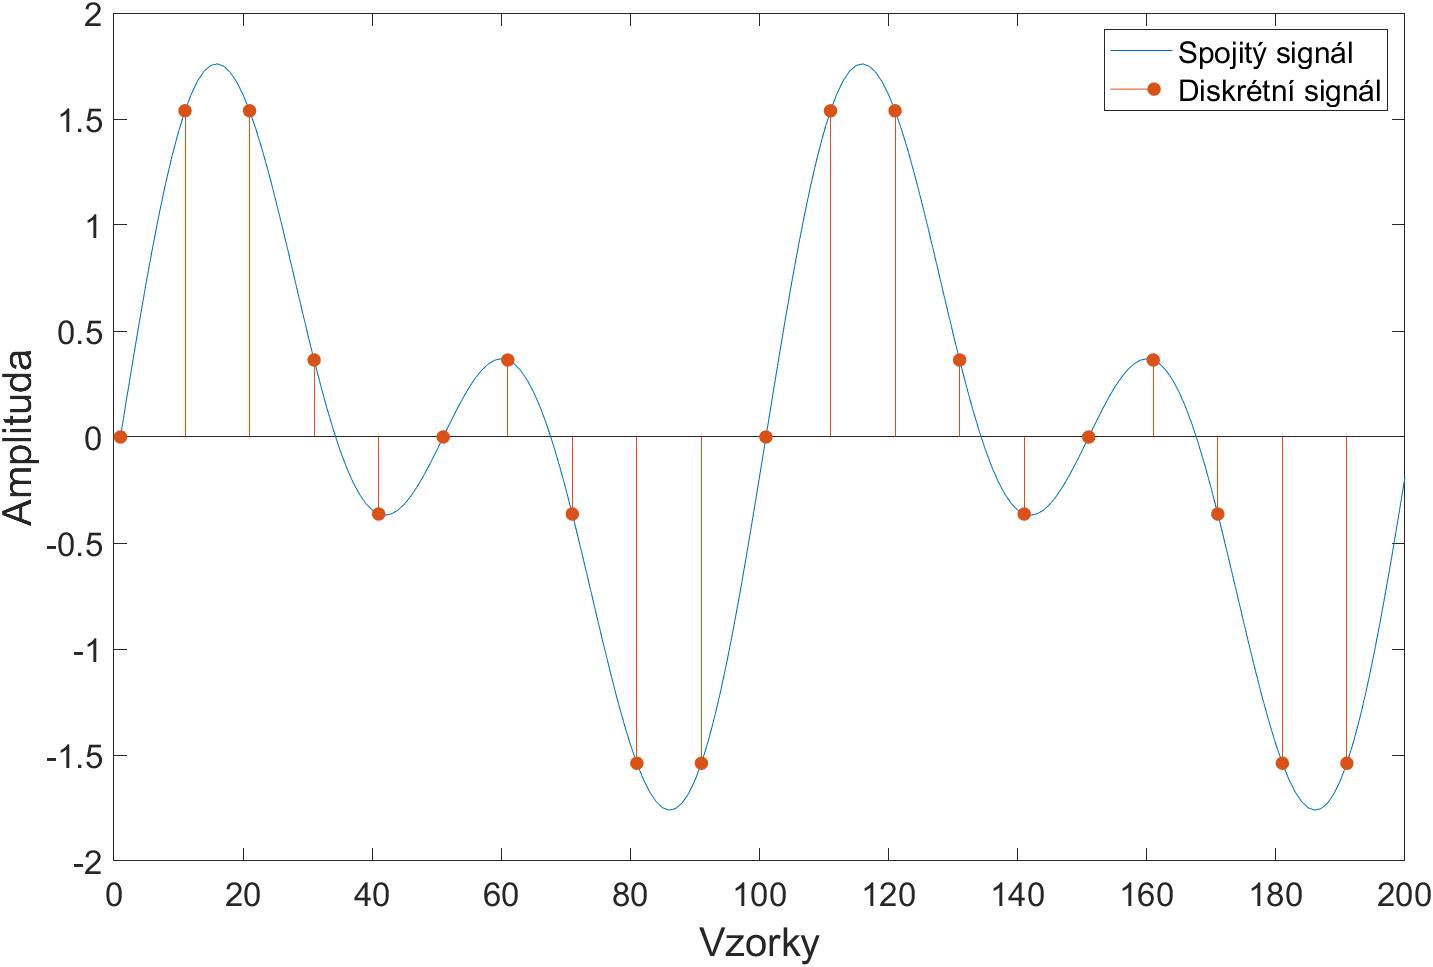
\includegraphics[width = 0.8\linewidth]{obrazky/Discrete_signal.png}
    \caption{Časově spojitý signál a diskrétní signál}
    \label{fig:Discrete_signal}
  \end{figure}

  Rovnice pro \acs{DFT} je potom zapsána v následujícím tvaru. 

  \begin{equation}
    X(k) = \hat{x}(k/N) = \sum_{n = 0}^{N - 1} x(n) exp(-2 \pi i k/N)
    \label{rov:DFT}
  \end{equation}

  Kde $ k \in [0:M - 1] = [0:N - 1] $ a $ M \in \mathbb{N}$.

  Ze strany výpočetní náročnosti je takto definovyný algoritmus neefektivní a výpočetně náročný.
  Při počítání Fourierova koeficientu $X(k)$ je zapotřebí velkého množství velké množství operací v řádu $N^2$.
  Proto pokud počet vzorků $N$ dosahuje většího množství je ve většině případů tento algoritmus příliš pomalý pro praktické využití.

  Počet potřebných operací může být výrazně redukován použitím efektivního algoritmu známého jako \acs{FFT} (\acl{FFT}).
  Na vytvoření\acs{FFT} se zasloužil Carl Friedrich Gauss a Joseph Fourier zhruba před dvěma sty let.
  Vynález tohoto algoritmu změnil své odvětví zpracování signálů a je dnes používán v miliardách telekomunikačních zařízeních.
  Ačkoliv je ve velké míře využíván v telekomunikacích, tak právě i ve zpracování a analýze zvukových signálů zabírá důležitou roli.

  Zjednodušeně \acs{FFT} využívá redundace napříč sinusovými signály různých frekvencní ke společnému výpočtu všech Fourierových koeficientů pomocí rekurze.
  Díky tomu je dosaženo snížení výpočetní náročnosti počtu operací z řádu $N^2$ na $N\log_2 N$.
  Například při použití vzorků $N = 2^10 = 1024$. \acs{FFT} vzžaduje $N\log_2N = 10240 $ operací namísto
  $N^2 = 1048576$ operací při použití \acs{DFT}. Jak je vidět snížení výpočetní náročnosti je velké a exponenciálně roste s větším počtem vzorků $N$.
  
  \subsection{STFT - Short-time Fourier transform}

  V roce 1946 Dennis Gabor představil \acs{STFT} jako potřebu zařazení frekvenčních složek do konkrétnímo času signálu.
  Fourierova transformace umožňovala převod signálu z časové oblasti do frekvenční ale nebylo zřejme v jakém časovém úseku signálu se získané fekvenční složky nachází.
  Hlavní myšlenkou \acs{STFT} je, že namísto analyzování celého signálu je signál analyzována pouze jeho malá část.
  Za tímto účelem je definována tzv. okénokvá funkce, která je nenulové pouze v malé části signálu.
  Analyzovaný signál je následně vynásoben vzniklou okénkovou funkcí a díky tomu vzniká malá nenulová části signálu dle okénkové funkce viz obr č. \ref*{fig:princip_stft}.
  Chceme li analyzovat signál v různých časech je tato funkce po signálu posouvána a následně se počítá Fourierova transformace pro každý výsledný okénkový signál.

  \begin{figure}[H]
    \centering
    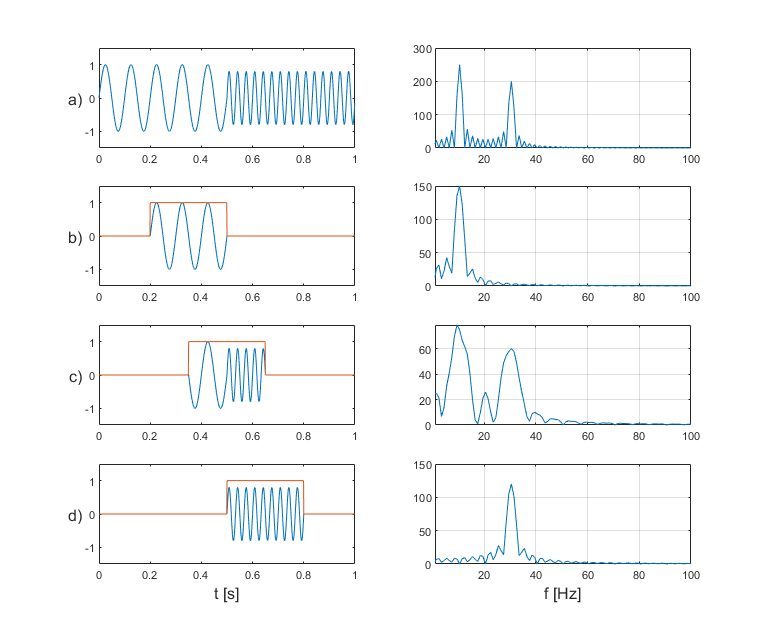
\includegraphics[width = 1\linewidth]{obrazky/STFT.png}
    \caption{Signál o délce $1 s$ s počáteční frekvencí $10 Hz$ a koncovou frekvencí $30 Hz$ \textbf{a)} Původní signál \textbf{b)} Signál s okénkem od $0,2 s$ do $0,5 s$ \textbf{c)} Signál s okénkem od $0,35 s$ do $0,65 s$ \textbf{d)} Signál s okénkem od $0,5 s$ do $0,8 s$};
    \label{fig:STFT}
  \end{figure}

  Na obrázku č. \ref*{fig:STFT} je graficky znázorněna myšlenka \acs{STFT}, která ukazuje výhodu přesného určení frekvenčních složek signálu v čase. 
  Signál je násoben obdelníkovou okénkovou funkcí ve třech místech.
  Tyto tři vzniklé signály jsou následně na sebe nezávazně transformovány do frekvenční oblasti.
  Z výsledků Fourierovy transformace lze vidět, že každá z těchto částí má jiné frekvenční spektrum.
  Pokud by bylo zapotřebí například určit přesný přechod mezi dvěma frekvencemi nacházejícími se v signálu. Lze spřesnit časové měřítko analýzy pomocí délky okénka.
  Tím ale dochází ke zmenšení přesnosti ve frekvenční oblasti.
  
  Na výsledku přesnosti analýzy poomcí \acs{STFT} závisí také tvar použité okénkové funkce.
  V obrázku č. \ref*{fig:STFT} je použito obdélníkového okénka které díky svým ostrým hranám zkresluje výsledek o nechtěné frekvenční složky.
  Existuje více tvarů okénkových funkcí pro odstranění nežádoucích složek.
  Například to jsou Kaise, Chebyshev, Hann a Haming a další.
  \cite{Time-frequency_distributions};

  %TODO: popsat parametry z knížky: dynamika intenzita a hlasitot, barva

  \subsection{Dynamika intenzita a hlasitost} \label{sec:Frekvence}

  Pojem \textbf{dynamika} je vyjadřuje jak hlasitost \uv{volume} zvuku stejně jako v notovém zápise udává hlasitost \uv{volume} přednesu.
  V notovém zápise je dynamika popsána symboly jako jsou například pianissimo \uv{\emph{pp}}, piano \uv{\emph{p}}, forte \uv{\emph{f}} a další.

  Naopak ve audiu je dynamika udána \textbf{hlasitostí \uv{loudness}} představována apmlitudou signálu nebo jeho efektivní hodnotou \acs{RMS} v čase.
  Při měření hlasitosi je pak využíváno pojmů \textbf{intenzita} zvuku a \textbf{akustický výkon}.
  Kde akustický výkon je definován jako kolik energie je vzduchem vyzářeno zvukovým vysílačem za jednotku času. Jednotkou je $[W]$
  A intenzita zvuku pak je definována jako množství energie, které projde jednotkovou plochou kolmou na směr šíření na jednotku času. Jednotkou pak je $[Wm^{-2}]$ \cite{intenzita_zvuku_definice}
  
  Z pohledu vnímání hlasitosti lidským uchem je rozsah vnímané intenzity zvuku v řádech bilionů. Práh slyšení činí $10^{-12} Wm^{-2}$ a práh bolesti je $10 Wm^{-2}$.
  Pro zmenšení tak velkého řádu je definována hladina intenzity zuvku v decibelech [$\textbf{dB}$]. Kde vztažnou hodnotou je práh slyšení $I_0 = 10^{-12} Wm^{-2}$.
  Hladina intenzity se vypočítá dle rovnice č. \ref*{rov:hladina_intenzity}

  \begin{equation}
    L_I = 10*log(\frac{I}{I_0})
    \label{rov:hladina_intenzity}
  \end{equation}

  \subsection{Barva} \label{sec:Barva}

  Hudebním vyjádření se za slovem barva zkrývá velmi komplexní sdružení atributů.
  Jedná se jak o psychologický tak hudební problém který je vnímán individuálně.
  \cite{The_perception_of_musical_timbre}

  Zdjednodušeně se barva definuje jako vlastnosti díky které je možné rozeznat tón o stejné výšce a hlasitosti zahraný na dva různé náastroje.
  Díky barvě je posluchač schopen rozeznávat různé zvuky nástrojů a typů interpretace.

  Jelikož je barva špatně kategorizovatelná fyzikálníma veličinama je většinou interpretována nedefinovanými slovy.
  Například popisujeme barvu jako jasnou, temnou, ostrou, čistou, teplou a další.

  Jedním z možných nástrojů pro analýzu barvy tónu je tvz. obálka tónu/signálu.
  Obálku signálu určuje amplituda signálu v čase viz obrázek č. ....%TODO: Přidat obrázek ADSR obálky
  Je rozdělena na 4 fáze a to jsou \textbf{Attack - náběh} určující začátek tónu například úder paličkou na blánu bubnu.
  V této fázi se nachází více ruchových složek z daného úderu a má velkou dynamiku.
  Následuje fáze s názvem \textbf{Decay - útlum}.
  Po hlasitém úderu amplituda signálu klesá a začíná převládat tonální složka. Decay udává dobu za kterou se signál z jeho maxima sníží na hodnotu sustain.
  \textbf{Sustain - podržení} je fáze ve které je zřetelný tón a stálá hlasitost. Rezonující blána bubnu.
  Poslední fází je \textbf{Release - uvolnění} při kterám dochází k poklesu hlasitosti zdroje zvuku až k uplnému utlumení.
  Například přiložení tlumítka na rezonující strunu.

  \begin{figure}[H]
    \centering
    \begin{subfigure}[b]{0.8\linewidth}
        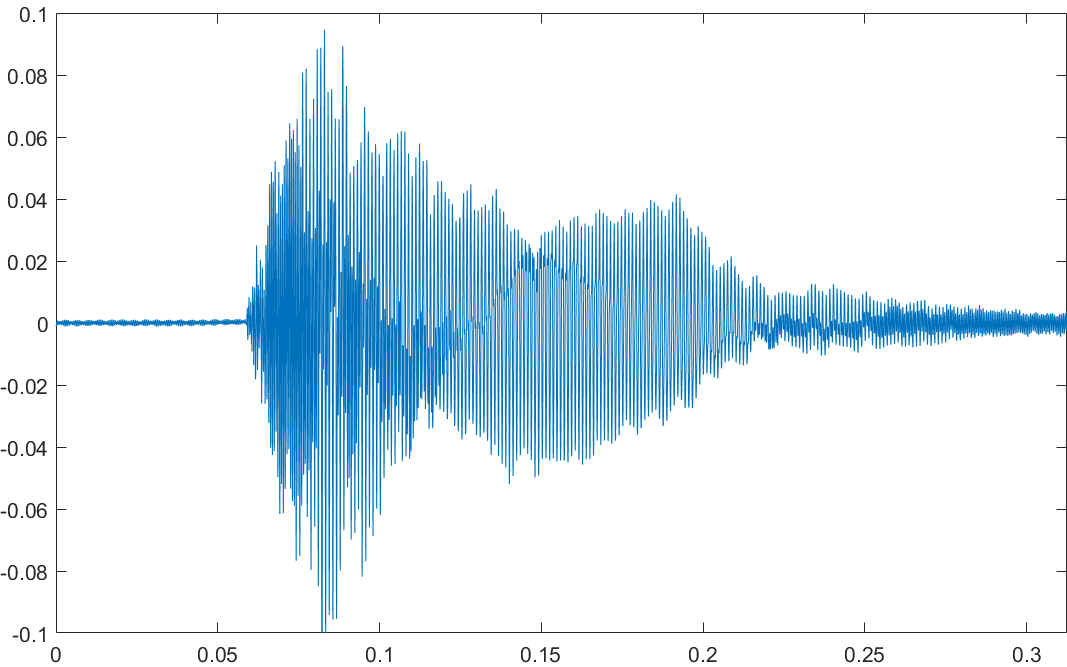
\includegraphics[width = \linewidth]{obrazky/Piano_tone_waveform.png}
        \caption{Amplituda tónu}
    \end{subfigure}
    \begin{subfigure}[b]{0.8\linewidth}
        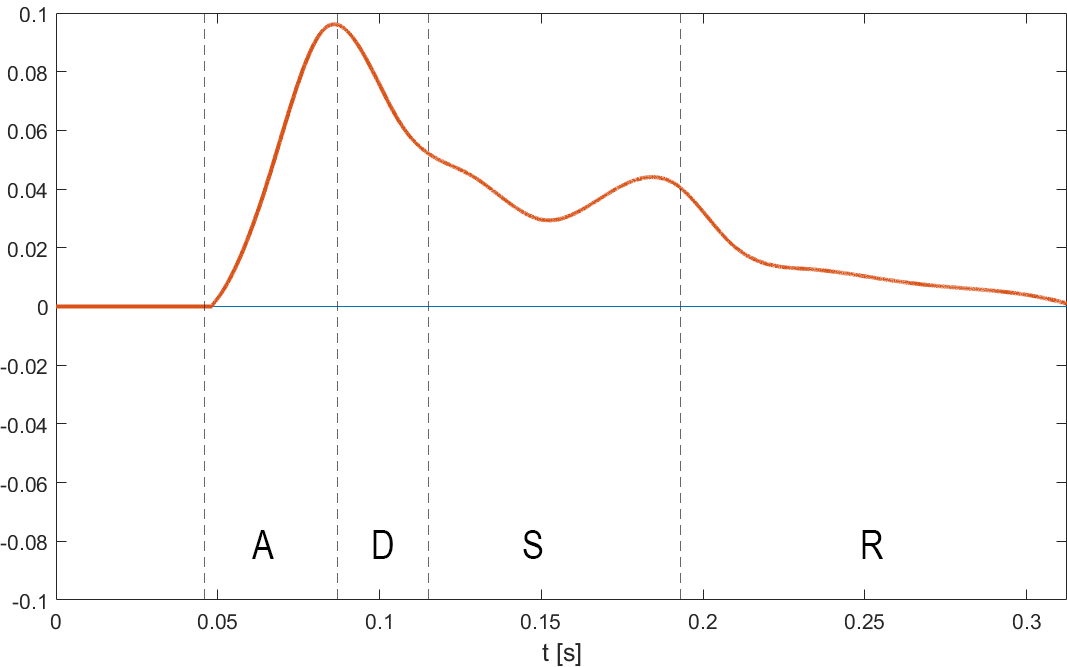
\includegraphics[width = \linewidth]{obrazky/Piano_tone_obalka.png}
        \caption{Obálka tónu}
    \end{subfigure}
    \caption{Tón A5 zahraný na klavír a jeho ADSR obálka}
    \label{fig:Bass_tone}
  \end{figure}

  Další informace o barvě signálu se nacházejí v jeho frekvenčním spektru. 
  Tón zahraný na hudební nástroj má svou fundamentální (nosnou) frekvenci nazávanou první harmonická frekvence udávající jeho výšku.
  Dle konstrukce nástroje se v signálu objevují násobky nosné frekvence.
  Tyto násobky představují vyšší harmonické složky tónu.
  Počet a amplituda vyšších harmonických složek má velký vliv na výslednou barvu tónu a je to hlavní důvod proč je lidské ucho schopné rozeznat stejný tón znějící na různé nástroje.

  %TODO: vložit obrázek

\section{Detekce tempa a dob}
\section{Klasifikace žánrů a nálady}

\section{Systém Spectoda}

\section{Hudební signál jako animace}